In run 3 of the LHC, it is envisaged that the luminosity for Pb-Pb collisions will increase significantly leading to an interaction rate of 50 kHz for Pb-Pb data taking, while p-p and p-Pb collisions will have an interaction rate of up to 1 MHz at Point 2. Many of the physics signals of interest to ALICE are complex to separate, and therefore not amenable to hardware triggers. Instead, ALICE intends to read out continuously, applying a minimum bias trigger to the data stream to flag events and using sophisticated filters on fully reconstructed events. In order to achieve this, most but not all detectors will upgrade to continuous readout. Adapting to continuous readout necessitates a new trigger system, but, as not all detectors will be upgraded, the new system must retain backwards compatibility.

\subsubsection{Requirements of the Trigger System}
The trigger system must have two simultaneous modes of running, one for triggered and one for continuous readout detectors, and deliver triggers at three different latencies (referred to as LM, L0, and L1) depending on the timing requirements of each detector. The system is required to have no deadtime i.e. be capable of receiving triggers every bunch-crossing, and is able to transmit trigger data at a rate of up to 9.6 Gbps. Due to the different requirements of detectors, the system will employ three types of optical trigger distribution. In addition, the system must monitor the status of all Common Readout Units (CRUs) and be able to reduce or stop their readout rate if CRU buffers become full.

\subsubsection{Trigger Hardware and Interfaces}
As with the trigger system employed in Runs 1 and 2 \cite{Aamodt:2008zz}, the upgraded system will be situated in the experimental cavern and consist of a Central Trigger Processor (CTP), which distributes and receives signals using up to 18 Local Trigger Units (LTUs), one for each detector. The LTUs may be decoupled from the CTP and used to emulate CTP signals for testing purposes. The emulation of trigger sequences using the LTU is an important part of the testing and commissioning of detector electronics. The CTP functionality is accommodated on a single triple-width 6U VME board using the VME format for power supply only. The board uses $+$5V/10A and $\pm$12V/1A from the VME power supply and generates the other required voltages using DC-DC converters. The board is equipped with a Xilinx Kintex Ultrascale FPGA (XCKU060-2FFVA1156E), two 1GB DDR4 memories, two Si5345 PLLs, an FME-HPC connector, two six-fold SFP+ cages and a single SFP+ cage, and two UCD90120A power controllers. The LTU and CTP boards are identical except the LTU boards use the slightly less powerful Xilinx Kintex Ultrascale FPGA (XCKU040-2FFVA1156E) and a smaller flash memory as they require less logic than the CTP.

The CTP board will utilise a FMC CTP mezzanine card with a total of 72 LVDS connections, which can be configured for either input or output. Two differential links will be used for clock signals, 45 for trigger inputs (10 LM, 18 LO, and 17 L1), four for BUSY inputs, and two for direct LM trigger outputs (for detectors requiring the fastest possible trigger); leaving 19 spare LVDS connections. The FMC connector will not be used for most LTUs but a commercial FMC S-18 card with seven usable SFP+ connection is used for detectors requiring extra optical links.

An important feature of the design is that all data interfaces for the board are via the front panel, rather than the VME bus. The available interfaces are:
\begin{enumerate}
\item A USB-JTAG connector for configuring the FPGA and FMC card. In the ALICE cavern, the JTAG will be connected to the Trigger PC located on the surface via a USB to Ethernet module (Anywhere USB).
\item A Power Management (PMbus) connector.
\item Eight LEMO 00 b ECL connectors.
\begin{itemize}
\item One for the LHC bunch-crossing (BC) signal,
\item one for the LHC Orbit signal,
\item two outputs for an oscilloscope,
\item two for TTC-A and TTC-B output used for the legacy RD12 (Run 1) Trigger, Timing and Control (TTC) system,
\item one for an input pulser, and one spare.
\end{itemize}
\item Five LVDS LEMO connectors.
\begin{itemize}
\item Two for LVDS trigger outputs,
\item two for BUSY in and BUSY out signals, and
\item one for fast LM trigger input
\end{itemize}
\item A SFP+ optical connector for IPbus (used for control and monitoring of the board); 
\item Twelve SFP+ optical links (plus an additional seven if using the FMC card in LTU configuration). 
\item 72 LVDS connectors via the CTP FMC card (in CTP configuration)
\end{enumerate}
     
\subsubsection{Trigger Protocol and Data Format}
The main minimum bias trigger will be delivered to the CTP by the FIT detector but the ZDC, TOF, EMCAL, and PHOS detectors will also deliver trigger inputs. Trigger inputs are aligned and synchronized to the local BC clock by the CTP and trigger logic is applied, using a lookup table, to produce trigger signals. The CTP will generate a hardware trigger with three possible available latencies (referred to as LM, L0, and L1) to all detectors with continuous readout and detectors without continuous readout that are not busy and will have the ability to partition the detectors into up to 14 detector clusters. The CTP will also be able to deliver software and calibration triggers. The maximum latency for the trigger input signals to reach the CTP are 425ns, 1200ns, and 6100ns for LM, L0, and L1 respectively.

The CTP communicates with the LTUs via the upgraded TTC-PON optical system \cite{Mendes:2017aok}, which allows two-way data traffic. The LTUs deliver the triggers to detectors in three ways. Detectors not upgrading their FEE will have trigger data sent via the (Run 1) TTC system \cite{Taylor:592719}, directly to their FEE. Most of the detectors being upgraded will receive trigger data via a TTC-PON optical link to their Common Readout Units (CRUs) but some will require a direct link to their FEEs via GBT \cite{Baron:1236361}. The central trigger system is designed to be flexible enough to accommodate the requirements of all ALICE detectors and a genral overview fo the trigger system is shown in Figure \ref{fig:systemoverview}.
\begin{figure}
\centering
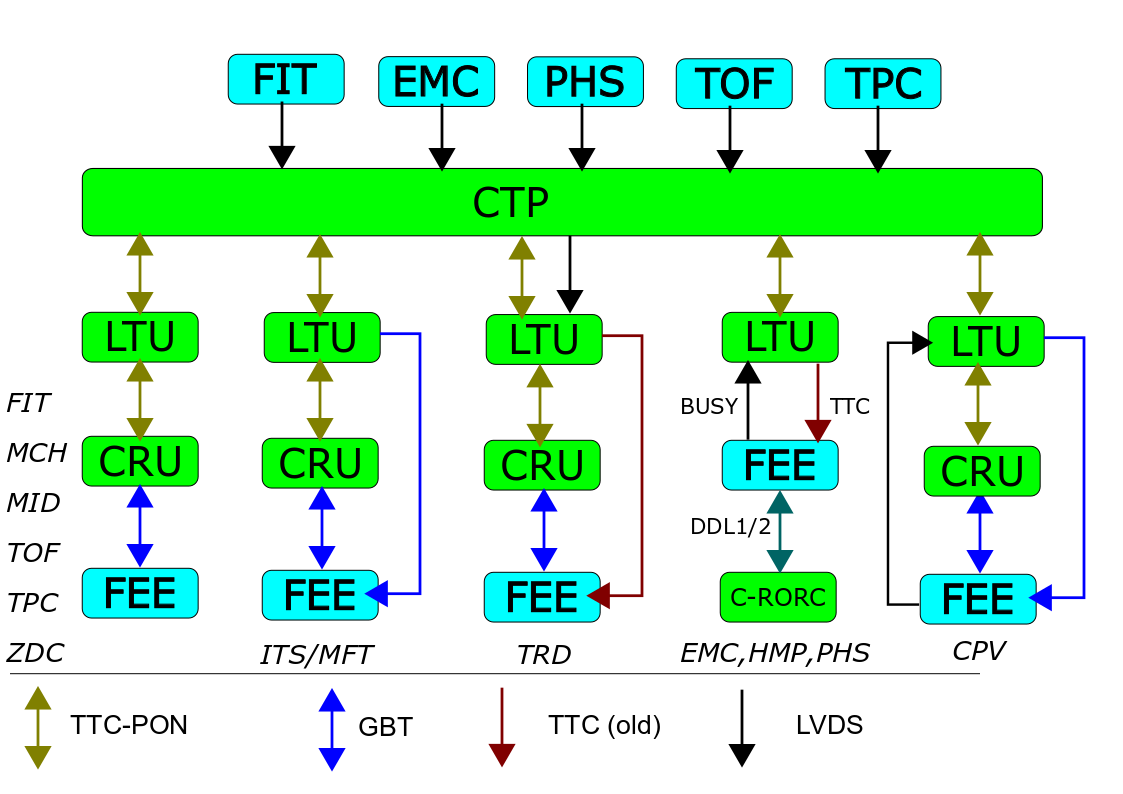
\includegraphics[width=0.7\textwidth]{CTSdistribution2.png}
\caption{\label{fig:systemoverview} Trigger System Overview. }
\end{figure}


As with the original CTP, many internal counters, including trigger inputs and sub-detector BUSY signals, will be monitored continually and this information will be read-out via the optical SFP+ link to the DAQ. The CTP will also incorporate a snapshot memory, which has proved useful in Runs 1 and 2. The 2GB of DDR4 memory on the CTP board will enable the CTP to take snapshots for 109 bunch crossings.  

% something on trigger data format

The trigger message (data) transmitted to the CRUs and the detector Front Ends (FE) consists of 77 bits arranged as follows: trigger type (32 bits), event identification (44 bits), and trigger type data valid bit. The event identification consist of an LHC orbit counter (32 bits) and bunch crossing counter (12 bits).
The trigger type valid bit indicates that the trigger field is valid, i.e. it is the OR of all Trigger Type bits. 
The ORBIT and BCID fields are always valid. 

% HB triggers
As well as sending triggers and trigger data every bunch crossing, dedicated time marks are provided by {\it HeartBeat triggers} (HB), sent nominally every LHC Orbit, containing the BC and Orbit numbers (HBid). HB triggers can be either a  HB accept (HBa) signalling CRUs to read out or a HB reject (HBr) signalling CRUs to discard data. Thus the HBa/HBr mechanism is logically similar to the BUSY protection in RUN2 (and for non-upgrading detectors). The decision on HBa/Hbr is made by the CTP according to the status of the CRUs.
A preloaded sequence of HBa and HBr triggers may be used to effectively downscale the continuous readout detectors if required. After receiving a HB trigger, each CRU ($\sim$ 500 in total) transmits a HB acknowledge message and their buffer status to the CTP, via their LTU. The CTP collects the HB acknowledge status of all CRUs, within a time-frame of eight Orbits and forms a HB map of the buffer statuses. The CTP maintains three HB maps at any time; one for the current HB and one for each of the two previous HB time frames but has a timeout of two Orbits for any given HB acknowledge. The CTP uses a pre-loaded set of conditions on the HB map to determine whether accept or reject the HB time-frame by transmitting a HBa or HBr trigger after the next HB timeframe (nominally one Orbit). Hence the HB map of CRU statuses is used to throttle the system using HBa and HBr messages. The trigger protocol and message flow is summarised in Figure \ref{fig:sigflow}.
\begin{figure}[h]
\centering
%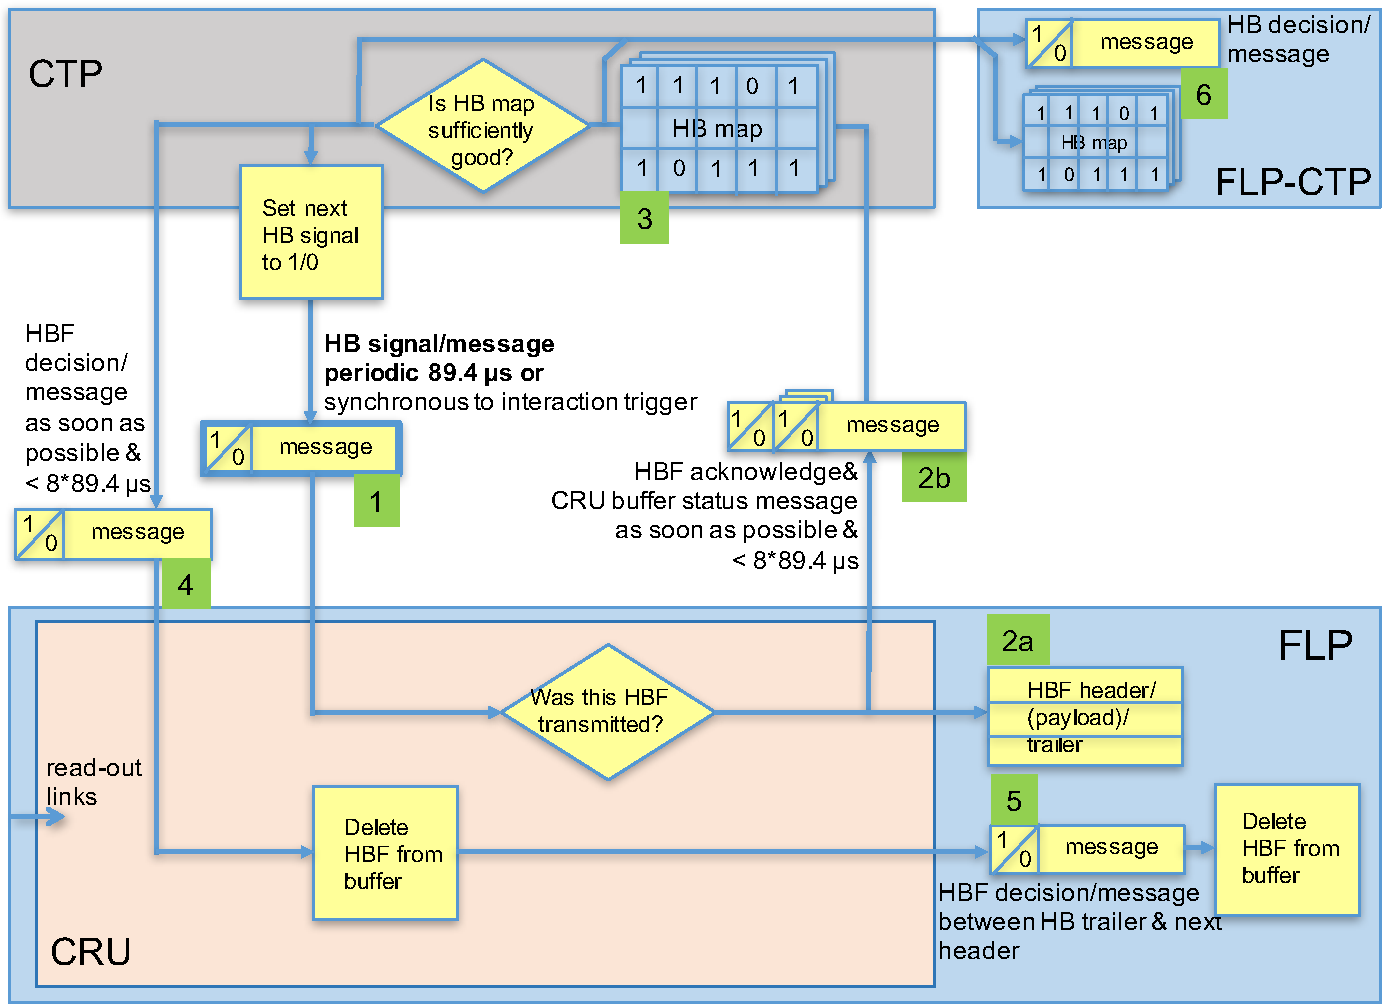
\includepdf[pages=-]{signalflow.pdf}
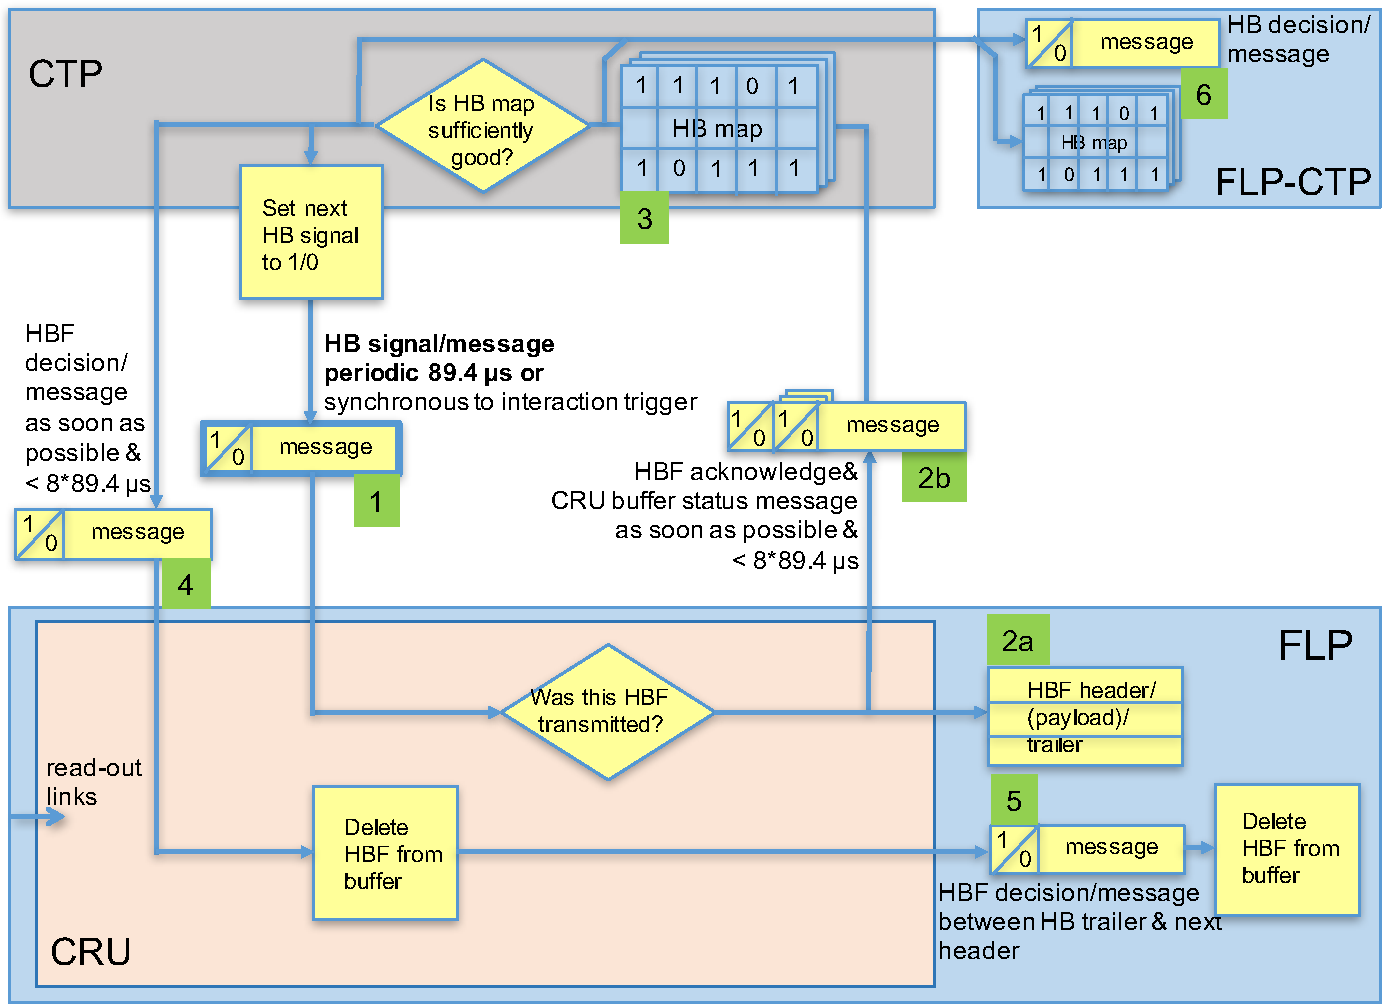
\includegraphics[width=0.7\textwidth]{signalflow.pdf}
\caption{\label{fig:sigflow} HeartBeat (HB) signal and message flow between CTP and CRUs. }
\end{figure}

% CTP readout
The information sent from CTP/LTU system to O2 is:
\begin{itemize}
\item copy of all triggers,
\item Trigger Input Mask (TIM: bitwise mask of trigger inputs in trigger data, 64 bits) and Detector Mask (DM: bitwise mask of detectors in trigger data, 18 bits) for every bunch crossing, 
\item HB map with payload of  
\begin{itemize}
\item HB id – Orbit (32 bits)  + BC id (12 bits)
\item 1 acknowledge bit and 2 buffer status bits per CRU
\end{itemize}
\end{itemize}
Hence the CTP presents itself, with respect to O2, almost as a  normal detector. The CTP sends, at every bunch crossing, the data containing the TIM ,DM  and HB mask to the O2 CTP CRU  and every detector LTU sends a  copy of all triggers to the O2 CTP CRU as well as the status of the CRU as seen by the LTU.

% software

The trigger boards are controlled via an IPbus interface \cite{Larrea:2015wra} and software for control and monitoring has been developed in python and C++ to take advantage of quick pythin development and C++ computing efficiency as necessary.

\subsubsection{Summary}
In summary, the central trigger system consists of the CTP and 18 LTU boards. The CTP distributes clock, heartbeats (HB), and triggers. The CTP receives HB acknowledge and status messages from the Common Readout Units (CRUs) and evaluates them. The LTUs in standalone mode emulates the CTP. The CTP is capable of deliverign triggers every bunch crossing, is backward compatible for non-upgraded detectors, and versatile enough to accommodate individual requires of detectors. 

